\documentclass{article}

\usepackage{fancyhdr}
\usepackage{extramarks}
\usepackage{amsmath}
\usepackage{amsthm}
\usepackage{amsfonts}
\usepackage{tikz}
\usepackage[plain]{algorithm}
\usepackage{algpseudocode}
\usepackage{enumitem}
\usepackage{pgfplots}

\usetikzlibrary{automata,positioning}

% Basic document settings
\topmargin=-0.45in
\evensidemargin=0in
\oddsidemargin=0in
\textwidth=6.5in
\textheight=9.0in
\headsep=0.25in

\linespread{1.1}

\pagestyle{fancy}
\lhead{\hmwkAuthorName}
\chead{\hmwkClass\ (\hmwkClassInstructor\ \hmwkClassTime): \hmwkTitle}
\rhead{\firstxmark}
\lfoot{\lastxmark}
\cfoot{\thepage}

\renewcommand\headrulewidth{0.4pt}
\renewcommand\footrulewidth{0.4pt}

\setlength\parindent{0pt}

% Pgfplots settings
\pgfplotsset{
    standard/.style={
        axis line style = thick,
        trig format=rad,
        enlargelimits,
        axis x line=middle,
        axis y line=middle,
        enlarge x limits=0.15,
        enlarge y limits=0.15,
        every axis x label/.style={at={(current axis.right of origin)}, anchor=north west},
        every axis y label/.style={at={(current axis.above origin)},anchor=south east},
        % grid=both,
        ticklabel style={font=\large, fill=white}
    }
}

% Create problem sections
\newcommand{\enterProblemHeader}[1]{
    \nobreak\extramarks{}{Problem \arabic{#1} continued on next page\ldots}\nobreak{}
    \nobreak\extramarks{Problem \arabic{#1}}{Problem \arabic{#1} continued on next page\ldots}\nobreak{}
}

\newcommand{\exitProblemHeader}[1]{
    \nobreak\extramarks{Problem \arabic{#1}}{Problem \arabic{#1} continued on next page\ldots}\nobreak{}
    \stepcounter{#1}
    \nobreak\extramarks{Problem \arabic{#1}}{}\nobreak{}
}

\setcounter{secnumdepth}{0}
\newcounter{partCounter}
\newcounter{homeworkProblemCounter}
\setcounter{homeworkProblemCounter}{1}
\nobreak\extramarks{Problem \arabic{homeworkProblemCounter}}{}\nobreak{}

% Homework problem environment
\newenvironment{homeworkProblem}[2][-1]{
    \ifnum#1>0
        \setcounter{homeworkProblemCounter}{#1}
    \fi
    \section{Problem \arabic{homeworkProblemCounter}: #2}
    \setcounter{partCounter}{1}
    \enterProblemHeader{homeworkProblemCounter}
}{
    \exitProblemHeader{homeworkProblemCounter}
}

% Homework details
\newcommand{\hmwkTitle}{Problem Set\ \#3}
\newcommand{\hmwkDueDate}{October 20, 2024}
\newcommand{\hmwkDueTime}{10:00pm}
\newcommand{\hmwkClass}{Macroeconomics}
\newcommand{\hmwkClassTime}{Section 101}
\newcommand{\hmwkClassInstructor}{Prof. Barnichon}
\newcommand{\hmwkAuthorName}{\textbf{Zachary Brandt}}

% Title page
\title{
    \vspace{2in}
    \textmd{\textbf{\hmwkClass:\ \hmwkTitle}}\\
    \normalsize\vspace{0.1in}\small{Due\ on\ \hmwkDueDate\ at \hmwkDueTime}\\
    \vspace{0.1in}\large{\textit{\hmwkClassInstructor\ \hmwkClassTime}}
    \vspace{3in}
}

\author{\hmwkAuthorName}
\date{}

% Various helper commands 

\renewcommand{\part}[1]{\textbf{\large Part \Alph{partCounter}}\stepcounter{partCounter}\\}

% Useful for algorithms
\newcommand{\alg}[1]{\textsc{\bfseries \footnotesize #1}}

% For derivatives
\newcommand{\deriv}[1]{\frac{\mathrm{d}}{\mathrm{d}x} (#1)}

% For partial derivatives
\newcommand{\pderiv}[2]{\frac{\partial}{\partial #1} (#2)}

% Integral dx
\newcommand{\dx}{\mathrm{d}x}

% Alias for the Solution section header
\newcommand{\solution}{\textbf{\large Solution}}

% Probability commands: Expectation, Variance, Covariance, Bias
\newcommand{\E}{\mathrm{E}}
\newcommand{\Var}{\mathrm{Var}}
\newcommand{\Cov}{\mathrm{Cov}}
\newcommand{\Bias}{\mathrm{Bias}}

\begin{document}

\maketitle

\pagebreak

\begin{homeworkProblem}[1]{Recovering from a War}
    Consider the basic Solow model with constant technology and constant population. Recall that the
    key equations of this model are
    
    \begin{enumerate}[topsep=15pt]
        \item[(1)] \:\:\: $Y_t = \Bar{A}K_t^{1/3}\Bar{L}^{2/3}$
        \item[(2)] \:\:\: $I_t = \Bar{s}Y_t$
        \item[(3)] \:\:\: $C_t = Y_t-I_t$
        \item[(4)] \:\:\: $K_{t+1} = K_t+I_t-\Bar{d}K_t$
    \end{enumerate}
    
    A) Suppose the economy starts off with a capital stock $K_0$. Using the Solow diagram, explain how
    the capital stock will evolve over time.
    \\ \\
    B) Now starting from a point where none of the exogenous variables have changed for a long period of time, suppose that a war occurs that destroys a large part of the capital stock. Using time series plots (i.e., plots with time on the x-axis and the variable being described on the y-axis), describe the evolution of the capital stock and output due to the war in qualitative
    terms. 
    \\ \\
    C) Recall that with competitive labor and capital markets the wage rate and the rental rate on capital will be given by
    \[
        \begin{split}
            \frac{2}{3}\Bar{A}\frac{K_t^{1/3}}{\Bar{L}^{1/3}} &= w_t
            \\
            \frac{1}{3}\Bar{A}\frac{\Bar{L}^{2/3}}{K_t^{2/3}} &= r_t
            \\
        \end{split}
    \]
    Using time series plots, describe the evolution of the wage rate and the rental rate on capital that occur due to the war in qualitative terms.

    \pagebreak
    \part
    
    Suppose the economy starts off with a capital stock $K_0$. Using the Solow diagram, explain how the capital stock will evolve over time.
    \\ \\
    \solution
    \\ \\
    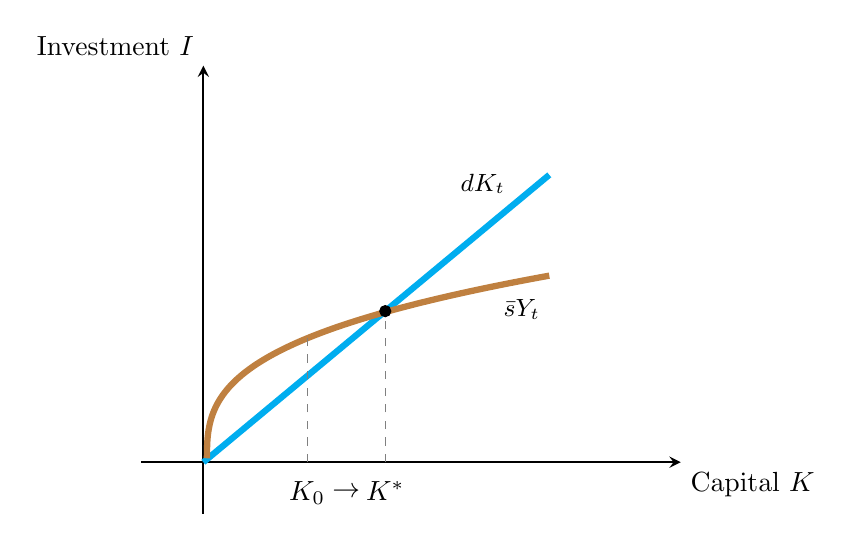
\begin{tikzpicture}
        \begin{axis}[standard,
                ytick=\empty,
                xtick=\empty,
                xticklabels={},
                yticklabels={},
                xlabel={Capital $K$},
                ylabel={Investment $I$},
                samples=1000, 
                xmin=0,
                xmax=3,
                ymin=0,
                ymax=
                3]
            \addplot[line width=0.8mm,cyan,domain={0:2.5}]{x};
            \addplot[line width=0.8mm,color=brown,domain={0:2.5}]{1.2*(x-0.025)^(1/3)};
            \addplot[dashed, gray, domain=0:1] coordinates {(1.31453,0) (1.31453,1.31453)};
            \node[anchor=center,label=south:{\textbf{$K^*$}}] at (axis cs:1.31453,0){};
            \addplot[dashed, gray, domain=0:1] coordinates {(0.75,0) (0.75,1.09027)};
            \node[anchor=center,label=south:{\textbf{$K_0$}}] at (axis cs:0.75,0){};
            \node[anchor=center,label=south:{$\rightarrow$}] at (axis cs:1.032265,-0.05){};
            
            \addplot[mark=* , color=black] coordinates {(1.31453, 1.31453)}; 
            
            \node[anchor=south east, color=black] at (axis cs:2.25, 2.25) {\small $dK_t$};
            \node[anchor=north west, color=black] at (axis cs:2.1, 1.5) {\small $\Bar{s}Y_t$};
        \end{axis}
    \end{tikzpicture}

    It will reach the equilibrium point after enough time periods where investment spending balances out capital depreciation. Or maybe actually golden rule level of capital

    \pagebreak
    \part

    Now starting from a point where none of the exogenous variables have changed for a long period of time, suppose that a war occurs that destroys a large part of the capital stock. Using time series plots (i.e., plots with time on the x-axis and the variable being described on the y-axis), describe the evolution of the capital stock and output due to the war in qualitative
    terms. 
    \\
    
    \solution 
    \\ \\
    If none of the exogenous variables have changed for a long period of time, then output and capital will have reached their equilibrium points. We can solve for the long run, or steady state, when $K_{t+1} = K_t = \overline{K}$. Substituting $\overline{K}$ into (4)
    \[
        \begin{split}
            \overline{K} &= \overline{K}+I_t-\overline{dK}
            \\
            \overline{dK} &= \overline{s}\overline{Y} \;\;\; \text{from (2)}
            \\
            \overline{dK} &= \overline{s}\overline{A}\overline{K}^{1/3}\overline{L}^{2/3} \;\;\; \text{from (1)}
            \\
            \overline{K}^{2/3} &= \frac{\overline{s}\overline{A}}{\overline{d}}\overline{L}^{2/3}
            \\
            \overline{K} &= \left( \frac{\overline{s}\overline{A}}{\overline{d}} \right)^{3/2}\overline{L}
        \end{split}
    \]

    Now, to find the time series plots we need to solve the differential equation $\frac{dK}{dt} = sAK^{1/3}L^{2/3} - dK$. General solutions to this nonlinear differential equation take the form
    \[
        \begin{split}
            K(t) = \overline{K} - \left( K_0 - \overline{K} \right)e^{-dt}
        \end{split}
    \]
    and subsituting in our expression for $\overline{K}$ this becomes
    \[
        \begin{split}
            K(t) = \left( \frac{\overline{s}\overline{A}}{\overline{d}} \right)^{3/2}\overline{L} - \left( K_0 - \left( \frac{\overline{s}\overline{A}}{\overline{d}} \right)^{3/2}\overline{L} \right)e^{-dt}        
        \end{split}
    \]

    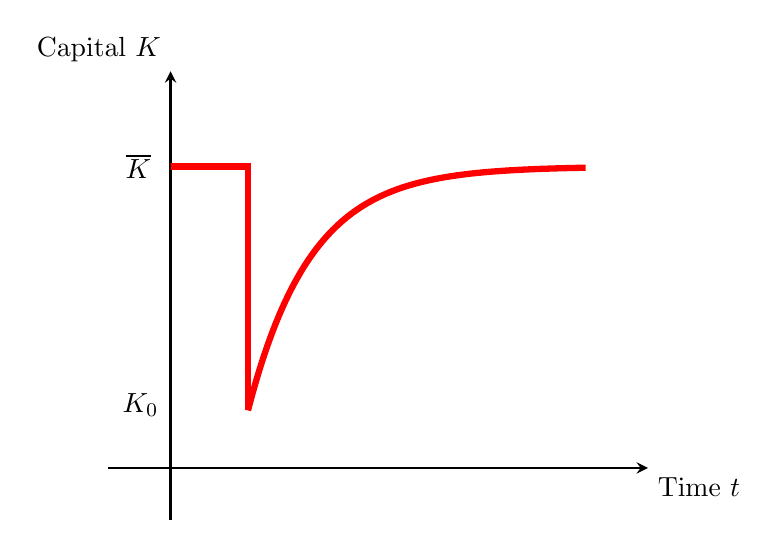
\begin{tikzpicture}
        \begin{axis}[standard,
                ytick=\empty,
                xtick=\empty,
                xticklabels={},
                yticklabels={},
                xlabel={Time $t$},
                ylabel={Capital $K$},
                samples=1000, 
                xmin=0,
                xmax=22,
                ymin=0,
                ymax=6]
            \addplot[line width=0.8mm,red,domain={0:4.104}]{5.243};
            \addplot[line width=0.8mm,red,domain={4.104:22}]{4.243+(1-4.243)*exp(-0.3*(x-5))+1};
            \addplot[line width=0.8mm,red,domain=0:5] coordinates {(4.104,1) (4.104,5.3)};
            \node[anchor=center,label=west:{$\overline{K}$}] at (axis cs:0,5.243){};
            \node[anchor=center,label=west:{$K_0$}] at (axis cs:0.4,1.1){};
        \end{axis}
    \end{tikzpicture}

    \pagebreak
    \part

    Recall that with competitive labor and capital markets the wage rate and the rental rate on capital will be given by
    \[
        \begin{split}
            \frac{2}{3}\Bar{A}\frac{K_t^{1/3}}{\Bar{L}^{1/3}} &= w_t
            \\
            \frac{1}{3}\Bar{A}\frac{\Bar{L}^{2/3}}{K_t^{2/3}} &= r_t
            \\
        \end{split}
    \]
    Using time series plots, describe the evolution of the wage rate and the rental rate on capital that occur due to the war in qualitative terms.
    \\

    \solution
    \\ \\
    First we need to find the long run equilibrium wage rate and rental rate on capital. Substituting $\overline{K}$ into the 
    equations for $w_t$ and $r_t$ we get

    \[
        \begin{split}
            \overline{w} &= \frac{2}{3}\Bar{A}\frac{\left( \left( \frac{\overline{s}\overline{A}}{\overline{d}} \right)^{3/2}\overline{L} \right)^{1/3}}{\Bar{L}^{1/3}} = \frac{2}{3}\Bar{A}\left( \frac{\overline{s}\overline{A}}{\overline{d}} \right)^{1/2}
            \\ \\ 
            \overline{r} &= \frac{1}{3}\Bar{A}\frac{\Bar{L}^{2/3}}{\left( \left( \frac{\overline{s}\overline{A}}{\overline{d}} \right)^{3/2}\overline{L} \right)^{2/3}} = \frac{1}{3}\Bar{A}\left( \frac{\overline{d}}{\overline{s}\overline{A}} \right)
        \end{split}
    \]

    We can create the time series plots for the wage rate and the rental rate on capital by substituting in the expression for 
    $K(t)$ into the equations for $w_t$ and $r_t$

    \[
        \begin{split}
            w_t &= \frac{2}{3}\Bar{A}\frac{K_t^{1/3}}{\Bar{L}^{1/3}} = \frac{2}{3}\Bar{A}\frac{\left( \left( \frac{\overline{s}\overline{A}}{\overline{d}} \right)^{3/2}\overline{L} - \left( K_0 - \left( \frac{\overline{s}\overline{A}}{\overline{d}} \right)^{3/2}\overline{L} \right)e^{-dt} \right)^{1/3}}{\Bar{L}^{1/3}}
            \\ \\ 
            r_t &= \frac{1}{3}\Bar{A}\frac{\Bar{L}^{2/3}}{K_t^{2/3}} = \frac{1}{3}\Bar{A}\frac{\Bar{L}^{2/3}}{\left( \left( \frac{\overline{s}\overline{A}}{\overline{d}} \right)^{3/2}\overline{L} - \left( K_0 - \left( \frac{\overline{s}\overline{A}}{\overline{d}} \right)^{3/2}\overline{L} \right)e^{-dt} \right)^{2/3}}
        \end{split}
    \]


    \begin{tikzpicture}
        \begin{axis}[standard,
                ytick=\empty,
                xtick=\empty,
                xticklabels={},
                yticklabels={},
                xlabel={Time $t$},
                ylabel={Wage Rate $w$},
                samples=1000, 
                xmin=0,
                xmax=22,
                ymin=0,
                ymax=3]
            \addplot[line width=0.8mm,red,domain={0:4.104}]{2.414};
            \addplot[line width=0.8mm,red,domain={2.104:22}]{(1/1.145)*(4.243+(-3.243)*exp(-0.3*(x-5)))^(1/3)+1};
            \addplot[line width=0.8mm,red,domain=0:5] coordinates {(4.104,1) (4.104,2.44)};
            \node[anchor=center,label=west:{$\overline{w}$}] at (axis cs:0,2.414){};
            \node[anchor=center,label=west:{$w_0$}] at (axis cs:0.4,1.1){};
        \end{axis}
    \end{tikzpicture}

    \begin{tikzpicture}
        \begin{axis}[standard,
                ytick=\empty,
                xtick=\empty,
                xticklabels={},
                yticklabels={},
                xlabel={Time $t$},
                ylabel={Wage Rate $w$},
                samples=1000, 
                xmin=0,
                xmax=22,
                ymin=0,
                ymax=1]
            \addplot[line width=0.8mm,red,domain={0:5}]{0.25};
            \addplot[line width=0.8mm,red,domain={5:22}]{(0.655)*(4.243+(-3.243)*exp(-0.3*(x-5)))^(-2/3)};
            \addplot[line width=0.8mm,red,domain=0:5] coordinates {(5,0.24) (5,0.655)};
            \node[anchor=center,label=west:{$\overline{r}$}] at (axis cs:0,0.25){};
            \node[anchor=center,label=west:{$r_0$}] at (axis cs:0.4,0.655){};
        \end{axis}
    \end{tikzpicture}

    
    
\end{homeworkProblem}

\pagebreak

\begin{homeworkProblem}[2]{Misallocation and TFP}
One lesson from the Solow model is that the determinants of long-run growth have to be found in total factor productivity $A_t$. Since $A_t$ is measured as the residual of a growth accounting decomposition,
TFP is often referred to as a measure of our ignorance. 
\\ \\
A recent insight from the academic literature on economic growth is that TFP can be affected by the allocation of factor inputs. This excercise will introduce you to this idea. 
\\ \\
Suppose output is produced using two tasks according to $Y=X_1^{\alpha}X_2^{1-\alpha}$. The tasks could be management vs. production work, manufacturing vs. services, or private sector work vs. public (e.g., regulatory, judicial, police) work. 
\\ \\
One unit of labor can produce one unit of either task, and the economy is endowed with L units of labor. Finally, suppose that the allocation of labor is such that a fraction $s$ of total labor works in the first task, and teh fraction $1-s$ works in the second task. 
\\ \\
A) Derive a production function of the form $Y=f(L)$, and derive an expression for TFP of this production function. 
\\ \\
B) Draw how TFP depends on the task allocation $s$ (recall $s \in [0,1])$.
\\ \\
C) What is the output maximizing allocation $s^*$? What happens to TFP then?
\\ \\
D) In many developing countries, taxes, poor management, information problems, or corruption can lead to a non-optimal allocation of tasks. How can this theory explain that some countries remain poorer than the US? 
    
\end{homeworkProblem}

\pagebreak

\begin{homeworkProblem}[3]{From Land to Fossil Energy}
    Consider the Malthus model of population growth with $\frac{N_{t+1}}{N_t} = (\frac{w_t}{w_s})$.
    \\ \\
    In the model we saw in class, we had the production function $Y_t = D^{\alpha}N_t^{1-\alpha}$, where land $D$ was fixed. In that economy, wages are stuck at subsistence levels in the long-run.
    \\ \\
    But imagine that we discover abundant (underground) fossil fuels so that land is only needed for food, making the land constraint effectively no longer binding so that we can assume that there is always enough land to grow in line with population. Instead, energy becomes a central part of the production process, and the function becomes the function $Y_t=E_t^{\gamma}L_{y,t}^{1-\gamma}$ with $\gamma < 1$ and $L_{y,t}$ is labor employed in the production of final goods $Y$.
    \\ \\
    Extracting energy from the ground requires labor and the production process for energy is $E_t=L_{e,t}$ with $L_{e,t} = sN_t$, where the fraction of the population devoted to energy extraction ($s$) is fixed. The rest of the population is devoted to production of $Y_t$, so $L_{y,t}=(1-s)N_t$.
    \\ \\
    It will be useful to define the term $g = (1-\gamma)(\frac{s}{1-s})^{\gamma}/w_s$. We assume that $g>1$.
    \\ \\
    A) Derive the equation for the wage rate $w_t$ in the final goods sector. Given the Malthus population dynamics $\frac{N_{t+1}}{N_t} = (\frac{w_t}{w_s})$, what is the population growth rate?
    \\ \\
    B) What is the economy's growth rate (i.e., the growth rate of $Y_t$)? What is the per capita growth rate (i.e., the growth rate of $Y_t/N_t$)?
    \\ \\
    C) How do workers fare in this economy compared to (i) a Malthusian economy, and (ii) a Solow economy (with constant $A_t$) that we saw in class?
    \\ \\
    D) Derive the level of energy extracted at each date $t$, i.e., derive an expression for $E_t$ as a function of initial conditions $N_0$ (the population at date 0). Derive the \textit{total} amount of energy extracted since time 0.
    \\ \\
    E) Fossil energy is in fact in finite supply on Earth. At which date $\tau$ will we have exhausted all fossil fuel? Derive an expression for $\tau$ as a function of model paramters. What will happen then to growth?
\end{homeworkProblem}

\end{document}
